\documentclass[journal, twoside, final]{IEEEtran}
\usepackage{geometry}
\usepackage{graphicx}
\usepackage{multirow}
\usepackage{caption}
\usepackage{float} 
% Author and title information
\title{Coronary Artery Disease (CAD) Prediction using Machine Learning Method with Ensemble Technique}
\author{
  \IEEEauthorblockN{Waqas Mehmood\IEEEauthorrefmark{1}\thanks{Capital University of Science and Technology, waaqasmehmood@gmail.com}} 
  \and
  \IEEEauthorblockN{Abdul Khaliq\IEEEauthorrefmark{2}\thanks{Capital University of Science and Technology, engg.abdulkhaliq@gmail.com}}
}

% Document content
\begin{document}

\maketitle

\begin{abstract}
Coronary Artery Disease (CAD) prediction is a crucial and challenging task in the medical field. CAD if detected at later stages can affect heart and blood vessels which can lead to blockage in veins and lead to a life threatening condition.  Our research paper encompasses the different classifications algorithms and final results are generated using ensemble technique which helped in generating perfect diagnosis of CAD. Ensemble methods including Logistic Regression, Naive Bayes Classifier, K-Nearest Neighbor (KNN), Decision Tree Classifier, Support Vector Machine and then Multi-model training was implemented to create a predictive model. Use of Machine Learning in CAD related risk assessment enables early detection and prevention life threatening impact of CAD.
\end{abstract}

\section{Introduction}
CAD is a health challenge at the global level. Disease of heart is jam or block your coronary clotting supply paths usually carried out by the development of greasy material called plaque. Coronary vein infection is additionally called coronary illness, ischemic coronary illness, and coronary disease. CAD ensues when plaque builds up in a patient's arteries as plaque continues to build [1].
ML predictive analysis is considered to be the best approach to prevent severe complications affecting both the heart and blood vessel. It can help in timely and precise identification of CAD which reduces risk of life threatening conditions due to heart disease. This research focuses on the application of machine learning classification algorithms, specifically use of ensemble techniques to predict CAD.
Ensemble techniques involve combining multiple ML algorithms to enhance overall predictive performance. This research explains the effectiveness of ensemble methods including Random Forests, Gradient Boosting and Multi-model training in constructing a robust predictive model for CAD. 
The primary purpose of this research is to assess the efficacy of ensemble learning in CAD prediction, which can help in early detection and accurate diagnosis. By incorporating multiple classification algorithms within the ensemble framework, we aim to enhance the model's sensitivity and specificity, leading to a more precise CAD prediction tool.
We used Cardiovascular Disease dataset containing 1024 patients’ record to train our model. The methodology section details data sources, preprocessing steps, and the implementation of ensemble techniques. The results and discussions focus on the performance of the proposed CAD prediction model, highlighting its potential impact on early detection and risk assessment. Our proposed algorithm is used for early prediction of CAD with a higher accuracy level.

\section{Literature Review}
Extensive work has already been done in this field yet there is gap for improvement. In previous studies, result accuracy on test data has never reached more than 88\%. Considering this a critical decease, accuracy must be increased. Table below contains the comparative analysis of accuracy result generated through previous work.


\begin{table*}[htbp]
  \caption{Summary of Papers}
  \centering
  \begin{tabular}{|c|c|p{4cm}|p{4cm}|c|}
    \hline
    \textbf{Year} & \textbf{Reference} & \textbf{Title of Paper} & \textbf{Classifier} & \textbf{Accuracy} \\
    \hline
    2018 & \cite{yekkala2017prediction} & Estimate of HD using ensemble learning and Subdivision Swarm Optimization & Naïve Bayes, K-nearest neighbor & 82.6\% \\
   \hline
    2019 &\cite{alizadehsani2019machine} & ML-based coronary artery disease diagnosis: An inclusive review & Ensemble model & 86.93\% \\
   \hline
    2019 & \cite{abdar2019performance} & HD prediction using machine learning analytical approach and Random forest algorithm & Random forest model & 76\% \\
   \hline
    2020 & \cite{mienye2020improved} & A data-driven approach for predicting the heart disease by using logistic regression & Logistic regression & 83.12\% \\
   \hline
    2020 & \cite{chang2019new} & A innovative intelligence system based on machine learning system for coronary heart disease prediction & XGBOOST & 82\% \\
   \hline
    2021 & \cite{shorewala2021early} & Design and Application of CAD prediction using NB & Naïve Bayes & 79\% \\
   \hline
    2022 & \cite{ahmad2022comparative} & CAD calculation using supervised type ML algorithm & RF, LG, SVM, KNN & 88\% and 85\% \\

    \hline
  \end{tabular}
\end{table*}

All the results mentioned in Table I, research work have used the Cleveland dataset in their studies. We also used it with another type of dataset obtained from the UCI dataset repository, having 14 attributes with 1024 different patient’s record
Some of above mentioned papers used ensemble technique which improved the overall accuracy but still there is gap for improvement in accuracy. The method we used to improve the overall accuracy is to use ensemble of algorithms generating satisfactory results on test data and ignore the algorithms for which accuracy and confusion matrix of test data is not good.

\section{Methods}
In machine learning, we can use different classifiers or their combinations to help us perform classification on given datasets. Here in our work, we want to predict the number of patients with or without heart disease by training our model on given dataset by running eight algorithms on our data set. The reason we use eight algorithms is that it will allow us to get better and more reliable predictions. We ensemble 5 classifier and performed hard voting classifier and then we ensemble 3 classifier with hard voting as shown in Fig 1.
\begin{figure}[htbp]
  \centering
  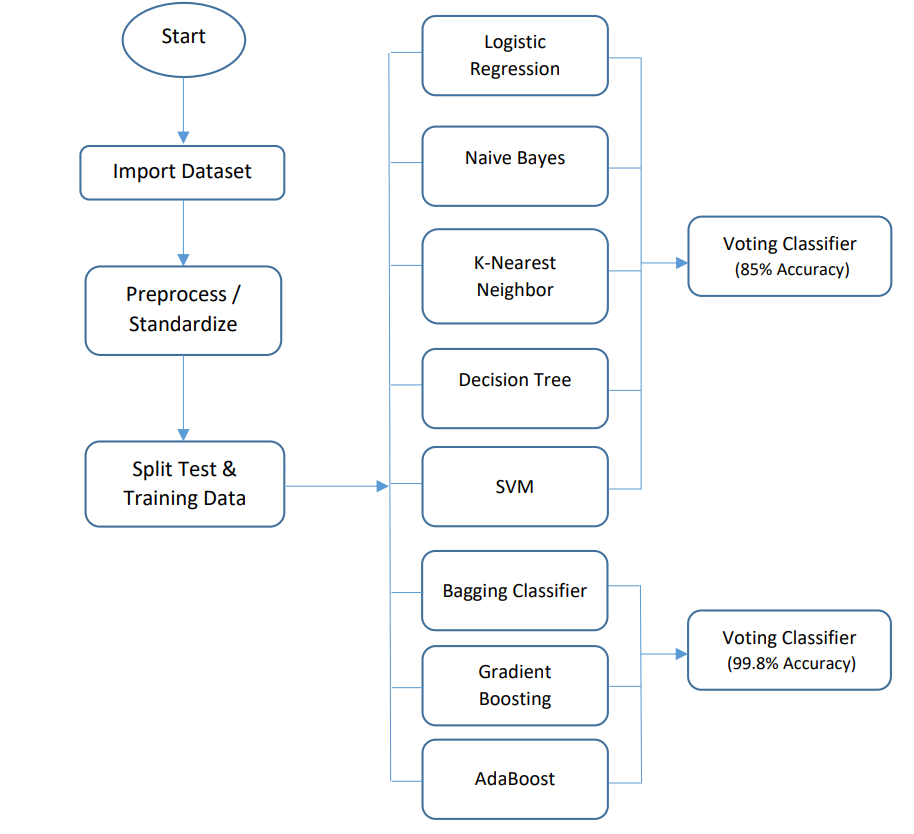
\includegraphics[width=0.5\textwidth]{flowchart.png} % relative path
  \captionsetup{justification=centering}
  \caption{Proposed Methodology}
\end{figure}


This dataset is obtained from UCI repository having 14 attributes with 1024 different patient’s record are shown in Table II. 

\begin{table}[htbp]
  \centering
  \caption{Attribute Description}
  \begin{tabular}{|p{0.2cm}|p{0.95cm}|p{1.9cm}|p{2.5cm}|}
    \hline
    {\textbf{No.}} &\centering{\textbf{Attribute}} & {\textbf{Description}} & {\textbf{Values}} \\
    \hline
    1 & \centering{age} & Age of patient & Age numeric values \\
 \hline
    2 & \centering{gender} & Gender & 1-Male, 0-Female \\
 \hline
    3 & \centering{C\_P} & Chest-pain & 1 = typ-ang, 2 = atypAng, 3 = non-ang \\
 \hline
    4 & \centering{trest\_bps} & Blood-pressure in rest & BP values \\
 \hline
    5 & \centering{CHOL} & Dietary fat & Cholesterol values \\
 \hline
    6 & \centering{F-B-S} & Sugar in blood & 1 = present, 0 = Absent \\
 \hline
    7 & \centering{restecg} & Echocardiography at rest & 1=Abnormal-ECG, 0=Normal \\
 \hline
    8 & \centering{oldpeak} & Exercise related to rest & Different values \\
 \hline
    9 & \centering{slope} & ST depression slope & 0, 1, 2 represent different slopes \\
 \hline
    10 & \centering{CA} & Vessels & 0, 1, 2, 3 values represent how your arteries are affected \\
 \hline
    11 & \centering{thal} & Thalassemia & 0, 1, 2, 3 represent colored Fluoroscopy vessels \\
 \hline
    12 & \centering{thalach} & Patient maximum heart rate & Heart rate values \\
 \hline
    13 & \centering{exang} & Angina with exercise & 1=present, 0=absent \\
 \hline
    14 & \centering{target} & Heart Disease & 1=effected person, 0=healthy \\
    \hline
  \end{tabular}
\end{table}
\section{Results}
After applying all the machine learning classifier on the dataset we get this results shown in the Table III.
Initially we used the Logistic Regression , Naive Bayes , KNN , DT and SVM classifiers to predict the Disease and there individual results are given in Table III. After that we combined these classifiers using hard voting classifier and predictions were not improved, So then we used Adaboost, Bagging and Gradient Boost ensemble techniques using Decision Trees and by using this method, the predicted results were significantly improved which are given in Table III. In our proposed methodology, we combined these ensemble classifiers using hard voting classifier and predicted results were perfect on test data. Results comparison is shown in Fig 2 in form of Accuracy, Precision, Recall and F1 Score. Results shows that VC-2 is giving the best result.
\begin{figure}[htbp]
  \centering
  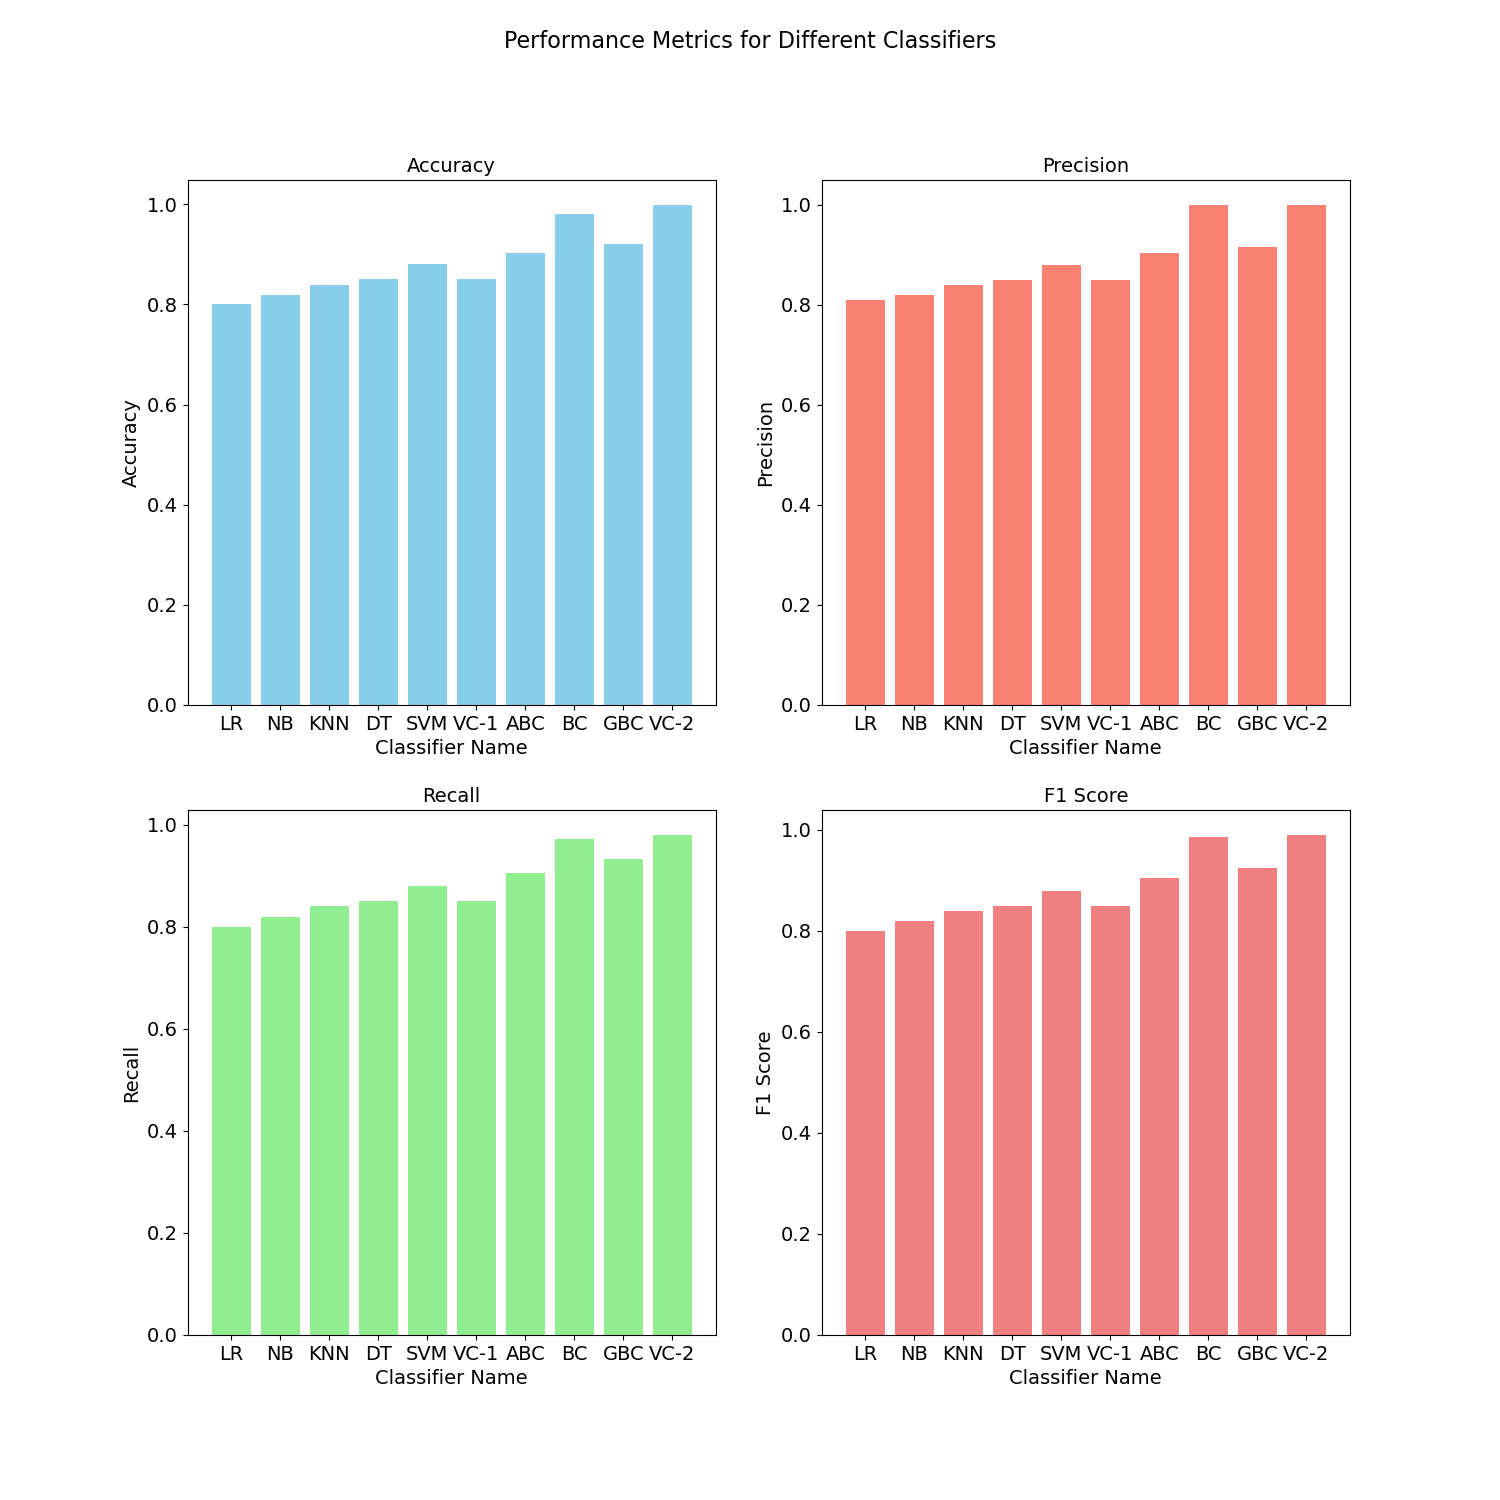
\includegraphics[width=0.6\textwidth]{performance_metrics.png} % relative path
  \captionsetup{justification=centering}
  \caption{Performace Comparison}
\end{figure}
\begin{table}[htbp]
  \centering
  \caption{Machine Learning Algorithms Results on Test Data}
  \begin{tabular}{|p{2cm}|p{0.95cm}|p{1cm}|p{1cm}|p{1cm}|}
    \hline
    \textbf{Classifier Name} & \textbf{Accuracy} & \textbf{Precision} & \textbf{Recall} & \textbf{F1 score} \\
    \hline
    {Logistic Regression} & {0.80} & {0.81} & {0.80} & {0.80} \\
 \hline
    Naive Bayes Classifier & 0.8195 & 0.82 & 0.82 & 0.82 \\
 \hline
    K-Nearest Neighbor & 0.8390 & 0.84 & 0.84 & 0.84 \\
 \hline
    Decision Tree Classifier & 0.85 & 0.85 & 0.85 & 0.85 \\
 \hline
    Support Vector Machine & 0.88 & 0.88 & 0.88 & 0.88 \\
 \hline
   {Voting Classifier with LR, NB, KNN, DT, SVM} & {0.85} & {0.85} & {0.85} & {0.85} \\
 \hline
    AdaBoost Classifier & 0.9024 & 0.9047 & 0.9047 & 0.9047 \\
 \hline
    Bagging Classifier & 0.98 & 1 & 0.9714 & 0.9855 \\
 \hline
    Gradient Boosting & 0.92 & 0.9158 & 0.9333 & 0.9247 \\
 \hline
   {Voting Classifier with AdaBoost, Bagging, GB} & {0.9987} & {1} & {0.98} & {0.99} \\
 \hline
   \textbf{Unseen Instance Test} : & \multicolumn{4}{|c|}{Correctly Classified} \\
    \hline
  \end{tabular}
\end{table}

\section{Conclusion}
In this research study, we have utilized eight machine learning algorithms on a dataset from the UCI repository, without implementing any feature selection technique.  Our research was conducted using the Python programming language with Jupiter Notebook. Initially, we applied our proposed classifiers to the datasets and calculated various metrics including accuracy, precision, recall, and F1 score. Subsequently, we combined five classifiers, namely Logistic Regression, Naive Bayes Classifier, K-Nearest Neighbor, Decision Tree Classifier and Support Vector Machine to evaluate the accuracies and compare the results with our ensemble model. Performance of model after ensemble was not significantly improved. After that we applied Random Forest, AdaBoost, Bagging and Gradient Boosting classifiers and ensemble them which significantly improved the results and accuracy on test data reached to 100\%. 

Bagging and Gradient Boosting classifiers and ensemble them which significantly improved the results and accuracy on test data reached to 100\%. 
Bagging and Gradient Boosting classifiers and ensemble them which significantly improved the results and accuracy on test data reached to 100\%. 
Bagging and Gradient Boosting classifiers and ensemble them which significantly improved the results and accuracy on test data reached to 100\%. Bagging and Gradient Boosting classifiers and ensemble them which significantly improved the results and accuracy on test data reached to 100\%. 

% Add references section
\bibliographystyle{plain}
\bibliography{references} % Replace 'references' with the name of your .bib file (without the extension)

\end{document}
